\section{Electro-Pneumatic System}

The electro-pneumatic system interfaces the engine and transmission module to the transmission's clutch and shift levers. The transmission controller portion of the engine and transmission module provide the control signals required to drive the electro-pneumatic system. The system design improves upon the previous generation discussed in Sec. \ref{sec:background_transmission} by targeting several of its noted deficiencies while reusing aspects of the design that worked well.

Rather than adopt a previously designed electro-pneumatic system, and attempt to improve performance simply by designing a controller, we opted to expand the scope of the design of this subsystem to include the design of the pneumatic system. This allowed us to expand the goals of this part of the project.

A fully-electronic design was initially considered, but later abandoned. The finalized design calls for an improved valving scheme and a closed-loop feedback system. A thorough literature review was conducted to determine the best control system possible. 

The clutch actuation design incorporates a novel \emph{pulse-width modulation} (PWM) control scheme to allow for precise positioning control. The shift actuation design is unchanged from the previous implementation. 

\subsection{Fully-Electronic Consideration}

The possibility of using a fully electronic actuation system with geared DC motors was carefully considered. The control of such a system would be far simpler, as linear approximate models of DC motors are readily available. Reasonably priced gear-head motors from several suppliers were investigated. It was determined that any suitable fully-electronic system would be far heavier than its pneumatic equivalent.

\subsection{Literature Review}

After deciding to keep a pneumatic actuation system, an improved valving scheme was proposed for the clutch, and sources of feedback were determined so that a closed-loop controller could be designed. Several academic papers were sourced that describe successful methods of pneumatic actuator control. \Citet{pneumatic_actuator} and \citet{adaptive_pneumatic} both use an electronically adjustable proportioning valve and a dual-acting cylinder. Proportioning valves are expensive (approximately \$300 from local suppliers) in comparison with binary solenoid valves (under \$50.)

Another approach by \citet{accurate_position} uses PWM signalled 3-way solenoid valves to control the air in and out of both sides of a dual-acting cylinder. By varying the duty cycle of the input signals, they were able to modulate the effective mass air flow rate through the cylinder ports: with the valve open, air would tend to flow from the high-pressure source into the cylinder, and with the valve closed, air would flow from the pressurized cylinder out through the exhaust port of the valve. This valving scheme allowed for a high degree of positional accuracy, however a large amount of air would be consumed during operation, as air is constantly being exhausted.

\subsection{Mechanical Components}

A diagram of the mechanical portion of the pneumatics system is shown in Fig. \ref{fig:pneumatics_design}. As in the previous design, an on-board compressed air tank is fitted with a pressure regulator, which regulates the system pressure to approximately $\unit{0.8}{\mega\pascal}$. Four solenoid valves controlled with signals $U_U$, $U_D$, $U_A$, and $U_B$ control the flow of air to and from 2 pneumatic actuators.

\begin{figure}[H]
	\centering
	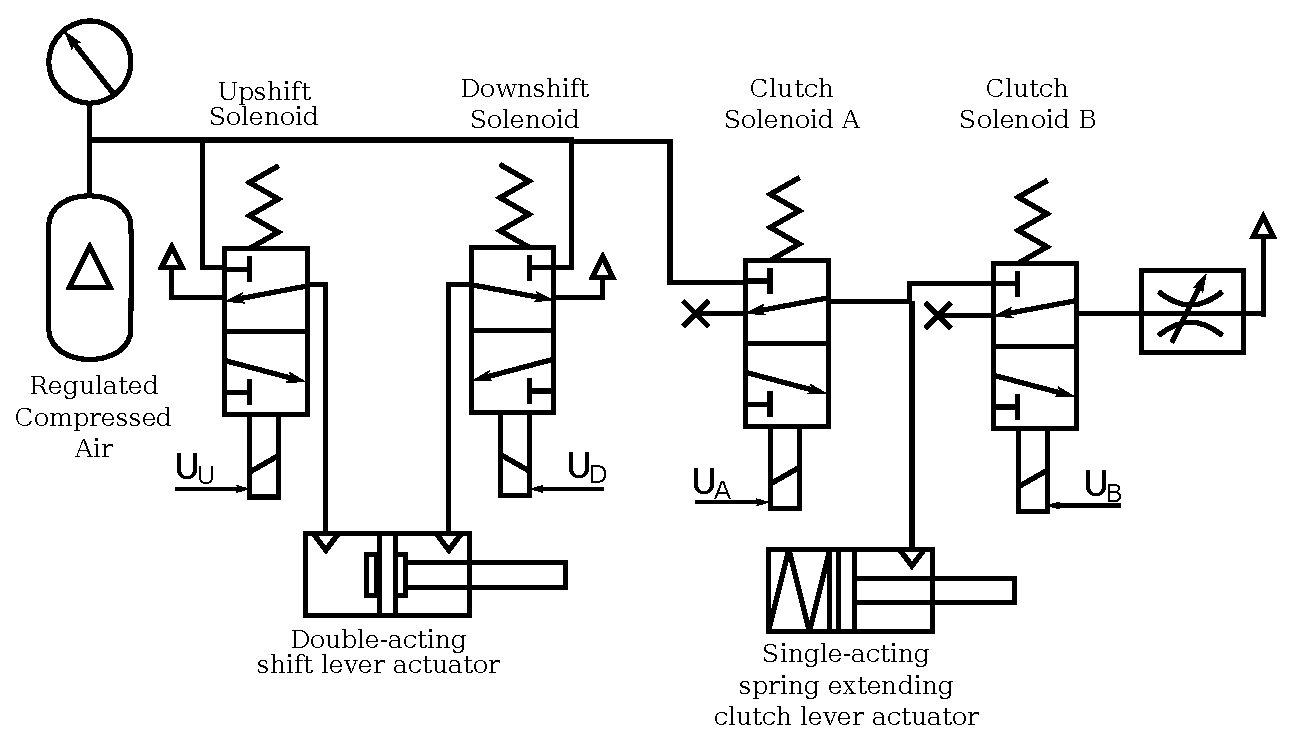
\includegraphics[scale=0.5]{design/figures/pneumatics}
	\caption{Component diagram of the electro-pneumatics system.}
	\label{fig:pneumatics_design}
\end{figure}

\subsection{Clutch Lever Actuation}
\nomenclature{PWM}{Pulse Width Modulation}
\nomenclature{$U_U$, $U_D$}{Output signals from the transmission controller to the upshift and downshift solenoids.}
\nomenclature{$U_A$, $U_B$}{Pulse width modulated output signals from the transmission controller to clutch solenoids A and B.}

The three approaches described in \cite{pneumatic_actuator, adaptive_pneumatic, accurate_position} considered the possibility of a highly dynamic load on the actuator. The load seen by the clutch actuator is far more predictable than the loads they expected and is only uni-directional. Since the vehicle is only equipped with a limited supply of air, conservation is a concern. Taking these factors into account, a single-acting cylinder with a return spring is specified for the clutch, and we propose a new valving scheme that allows a degree of controllability over the actuator while conserving as much air as possible.

The cylinder visible on the right of Fig. \ref{fig:pneumatics_design}, actuates the clutch lever. Precise control of the clutch is accomplished with fast solenoid valves \emph{Clutch Solenoid A} and \emph{Clutch Solenoid B}. These valves are signalled with a PWM scheme to modulate the average mass air flow rate into and out separately of the cylinder. Positional feedback for the clutch cylinder is provided by a combination of an internal magnet on the piston in the cylinder and a magnetic sensing membrane potentiometer.

Both clutch solenoids are shown as 3-way (with exhaust ports) valves in Fig. \ref{fig:pneumatics_design}, but the valves are used in a 2-way configuration with the exhaust ports plugged.  This results in the following operation:

\begin{enumerate}
  \item When the pulse width modulated control signal $U_A$ to Clutch Solenoid A is non-zero, the valve will open, and air will flow into the cylinder at a rate proportional to the duty cycle, disengaging the clutch.
  \item When pulses no longer arrive at Clutch Solenoid A (or the duty cycle of $U_A$ approaches 0), the valve remains closed, and any air in the cylinder is trapped. The clutch maintains is position.
  \item When the pulse width modulated control signal $U_B$ to Clutch Solenoid B is non-zero, the valve will open, and any pressure differential between the cylinder and atmosphere will cause air to flow out of the cylinder to atmosphere at a rate proportional to the duty cycle. The clutch springs and the cylinders' internal spring work to return the actuator position to rest, and the clutch engages.
\end{enumerate}

An additional adjustable flow rate control valve (visible on the far right in Fig. \ref{fig:pneumatics_design}) was added to the design to allow additional tuning for during clutch engagement. No air is wasted in disengaging the clutch and holding the position because the fill and exhaust operations are separately controlled with two valves.

\subsection{Shift Lever Actuation}

The shift lever does not require the same level of control as the clutch, and as such the design of the valving has not changed over previous implementations. Two binary valves are used with a dual-acting cylinder. The first actuator (visible on the left of Fig. \ref{fig:pneumatics_design}) actuates the shift lever between 3 different positions: up-shift, down-shift, and rest-state. The transmission spring-loads the lever to automatically return to the rest-state, which is half-way through the actuator stroke. Applying pressure to one port will pull the lever up, and applying pressure to the other port will pull the lever down. 

Current gear position is determined with a potentiometer that is mechanically linked to the shift drum. Control and timing signals are generated by the engine and transmission module.

